\documentclass{beamer}

\usepackage[detect-weight,detect-family]{siunitx}
\sisetup{output-decimal-marker = {,}}
\sisetup{exponent-product = {\cdot}}
\sisetup{group-digits = none}
\sisetup{round-mode = figures}
\sisetup{round-precision = 4}
\sisetup{round-pad = false}

\usepackage{amsmath}
\usepackage{amssymb}
\usepackage{mathtools}
\usepackage{resizegather}
\usepackage{icomma}
\mathtoolsset{showonlyrefs}
\usefonttheme[onlymath]{serif}
\newcommand{\Prod}{\,}

\usepackage{graphicx}
\usepackage{epstopdf}
\usepackage{wrapfig}
\graphicspath{{../img/}}
\epstopdfsetup{outdir=./build/}

\usepackage{tabularx}
\usepackage{booktabs}

\addtobeamertemplate{navigation symbols}{}{
  \usebeamerfont{footline}
  \usebeamercolor[fg]{footline}
  \hspace{1em}
  \raisebox{1.4pt}[0pt][0pt]{\insertframenumber/\inserttotalframenumber}
}

\renewcommand{\Prod}{\,}

\title{Identificação de Sistema por Erro de Predição com Modelos Racionais}
\author{Guilherme de Paoli Beal}
\institute{
  Universidade Federal do Rio Grande do Sul
  \\
  Programa de Pós-Graduação em Engenharia Elétrica
  \\
  Aprendizado Supervisionado de Modelos Paramétricos
}
\date{Maio de 2023}

\begin{document}

{
\setbeamertemplate{navigation symbols}{}
\begin{frame}[noframenumbering,label={frame:title}]
  \titlepage
\end{frame}
}

\begin{frame}{Sistema}
  Sistema SISO, discreto, linear e invariante no tempo:
  \begin{gather}
    y(t) = G_0(q) \Prod u(t) + \nu(t)
    \\
    \nu(t) = H_0(q) \Prod e(t)
  \end{gather}
  \begin{itemize}
    \item[$t \in \mathbb{N}$] variável de tempo discreto
    \item[$q$] operador de avanço
    \item[$y(t)$] sinal de saída
    \item[$u(t)$] sinal de entrada
    \item[$\nu(t)$] ruído de medição desconhecido
    \item[$e(t)$] ruído branco
    \item[$G_0(q)$] função de transferência do sistema
    \item[$H_0(q)$] função de transferência do filtro
  \end{itemize}
\end{frame}

\begin{frame}{Modelos Racionais}
  \begin{itemize}
    \item[ARX] Autorregressivo com Entrada Externa, ou \emph{Autoregressive with Extra Input}
    \item[ARMAX] Autorregressivo com Média Móvel e Entrada Externa, ou \emph{Autoregressive Moving Average with Extra Input}
    \item[OE] Erro na Saída, ou \emph{Output Error}
    \item[BJ] Box-Jenkins
  \end{itemize}
  Formato genérico:
  \begin{gather}
    A(q) \Prod y(t) = \dfrac{B(q)}{F(q)} \Prod u(t) + \dfrac{C(q)}{D(q)} \Prod e(t)
  \end{gather}
\end{frame}

\begin{frame}{Modelos Racionais}
  \begin{gather}
    A(q) \Prod y(t) = \dfrac{B(q)}{F(q)} \Prod u(t) + \dfrac{C(q)}{D(q)} \Prod e(t)
    \\\Updownarrow\\
    y(t) = G(q) \Prod u(t) + H(q) \Prod e(t)
    \\\\
    G(q) = \dfrac{B(q)}{A(q) \Prod F(q)}
    \qquad
    H(q) = \dfrac{C(q)}{A(q) \Prod D(q)}
    \\\\
    \begin{aligned}
      A(q) &= 1 + a_1 \Prod q^{-1} + \dotsb + a_{n_a} \Prod q^{-n_a}
      \\
      B(q) &= q^{-n_k} \Prod \left(b_0 + b_1 \Prod q^{-1} + \dotsb + b_{n_b} \Prod q^{-n_b}\right)
      \\
      C(q) &= 1 + c_1 \Prod q^{-1} + \dotsb + c_{n_c} \Prod q^{-n_c}
      \\
      D(q) &= 1 + d_1 \Prod q^{-1} + \dotsb + d_{n_d} \Prod q^{-n_d}
      \\
      F(q) &= 1 + f_1 \Prod q^{-1} + \dotsb + f_{n_f} \Prod q^{-n_f}
    \end{aligned}
  \end{gather}
\end{frame}

\begin{frame}{Predição}
  \begin{gather}
    \hat{y}(t) = L_u(q) \Prod u(t) + L_y(q) \Prod y(t)
    \\\\
    \begin{aligned}
      L_u(q) &= \dfrac{G(q)}{H(q)}
      \\
      L_y(q) &= 1 - \dfrac{1}{H(q)}
    \end{aligned}
  \end{gather}
  Erro de predição:
  \begin{align}
    \varepsilon(t)
    &= y(t) - \hat{y}(t)
    \\
    &= \dfrac{y(t) - G(q) \Prod u(t)}{H(q)}
  \end{align}
  Erro quadrático médio:
  \begin{equation}
    J = \dfrac{1}{N} \Prod \sum_{t=0}^{N-1}{\left(\varepsilon(t)\right)^2}
  \end{equation}
\end{frame}

\begin{frame}{ARX}
  \begin{itemize}
    % \item $n_a$
    % \item $n_b$
    \item $n_c=0$
    \item $n_d=0$
    \item $n_f=0$
    % \item $n_k$
  \end{itemize}
  \begin{gather}
    G(q) = \dfrac{B(q)}{A(q)}
    \qquad
    H(q) = \dfrac{1}{A(q)}
  \end{gather}
  \begin{align}
    A(q) &= 1 + a_1 \Prod q^{-1} + \dotsb + a_{n_a} \Prod q^{-n_a}
    \\
    B(q) &= q^{-n_k} \Prod \left(b_0 + b_1 \Prod q^{-1} + \dotsb + b_{n_b} \Prod q^{-n_b}\right)
  \end{align}
  $J$ é quadrático nos parâmetros
\end{frame}

\begin{frame}{ARMAX}
  \begin{itemize}
    % \item $n_a$
    % \item $n_b$
    % \item $n_c$
    \item $n_d=0$
    \item $n_f=0$
    % \item $n_k$
  \end{itemize}
  \begin{gather}
    G(q) = \dfrac{B(q)}{A(q)}
    \qquad
    H(q) = \dfrac{C(q)}{A(q)}
  \end{gather}
  \begin{align}
    A(q) &= 1 + a_1 \Prod q^{-1} + \dotsb + a_{n_a} \Prod q^{-n_a}
    \\
    B(q) &= q^{-n_k} \Prod \left(b_0 + b_1 \Prod q^{-1} + \dotsb + b_{n_b} \Prod q^{-n_b}\right)
    \\
    C(q) &= 1 + c_1 \Prod q^{-1} + \dotsb + c_{n_c} \Prod q^{-n_c}
  \end{align}
  Generalização do ARX
\end{frame}

\begin{frame}{Ouput Error}
  \begin{itemize}
    \item $n_a=0$
    % \item $n_b$
    \item $n_c=0$
    \item $n_d=0$
    % \item $n_f$
    % \item $n_k$
  \end{itemize}
  \begin{gather}
    G(q) = \dfrac{B(q)}{F(q)}
    \qquad
    H(q) = 1
  \end{gather}
  \begin{align}
    B(q) &= q^{-n_k} \Prod \left(b_0 + b_1 \Prod q^{-1} + \dotsb + b_{n_b} \Prod q^{-n_b}\right)
    \\
    F(q) &= 1 + f_1 \Prod q^{-1} + \dotsb + f_{n_f} \Prod q^{-n_f}
  \end{align}
  Assume $\nu(t) = e(t)$
\end{frame}

\begin{frame}{Box-Jenkins}
  \begin{itemize}
    \item $n_a=0$
    % \item $n_b$
    % \item $n_c$
    % \item $n_d$
    % \item $n_f$
    % \item $n_k$
  \end{itemize}
  \begin{gather}
    G(q) = \dfrac{B(q)}{F(q)}
    \qquad
    H(q) = \dfrac{C(q)}{D(q)}
  \end{gather}
  \begin{align}
    B(q) &= q^{-n_k} \Prod \left(b_0 + b_1 \Prod q^{-1} + \dotsb + b_{n_b} \Prod q^{-n_b}\right)
    \\
    C(q) &= 1 + c_1 \Prod q^{-1} + \dotsb + c_{n_c} \Prod q^{-n_c}
    \\
    D(q) &= 1 + d_1 \Prod q^{-1} + \dotsb + d_{n_d} \Prod q^{-n_d}
    \\
    F(q) &= 1 + f_1 \Prod q^{-1} + \dotsb + f_{n_f} \Prod q^{-n_f}
  \end{align}
  Modelo mais livre
\end{frame}

\begin{frame}{Critério de Informação de Akaike}
  \begin{gather}
    \text{AIC} = N \Prod \log\left(J\right) + 2 \Prod k
    \\
    \text{AICc} = \text{AIC} + \dfrac{2 \Prod k \Prod \left(k + 1\right)}{N - k - 1}
  \end{gather}
  \begin{itemize}
    \item[$N$] Número de amostras
    \item[$J$] Erro quadrático médio de predição
    \item[$k$] Número de parâmetros no modelo
  \end{itemize}
\end{frame}

\begin{frame}{Dados}
  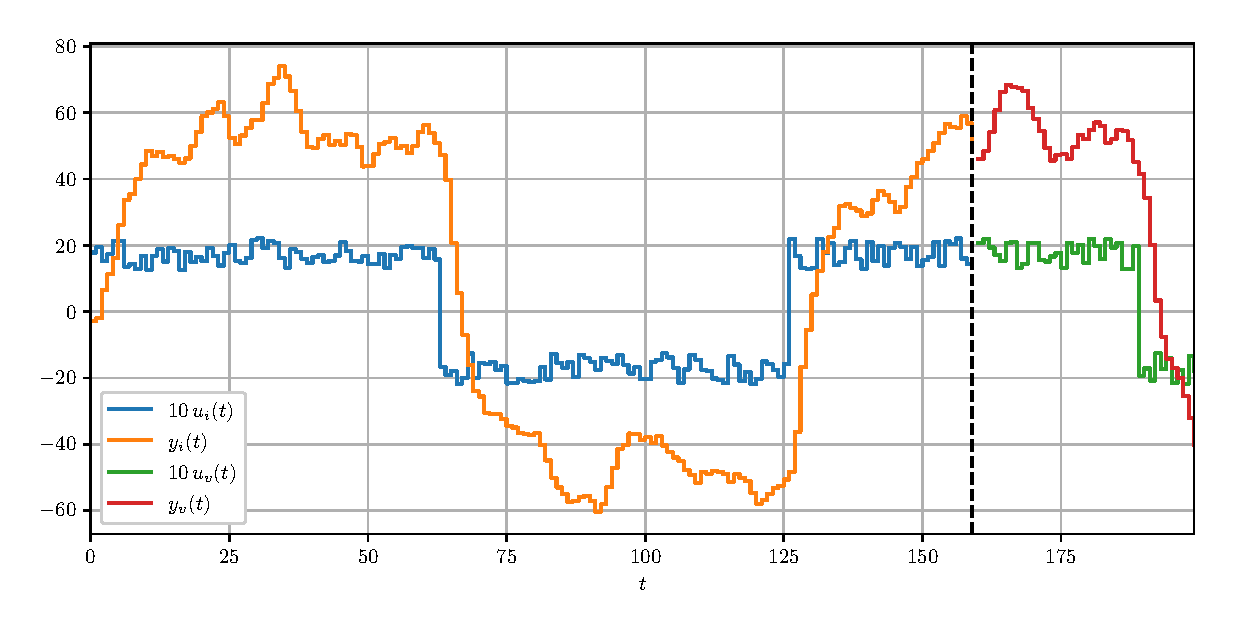
\includegraphics[width=\linewidth]{data_folded}
  Tracejado: divisão entre dados de identificação e de validação
\end{frame}

\begin{frame}{Dados - Espectro de Amplitude}
  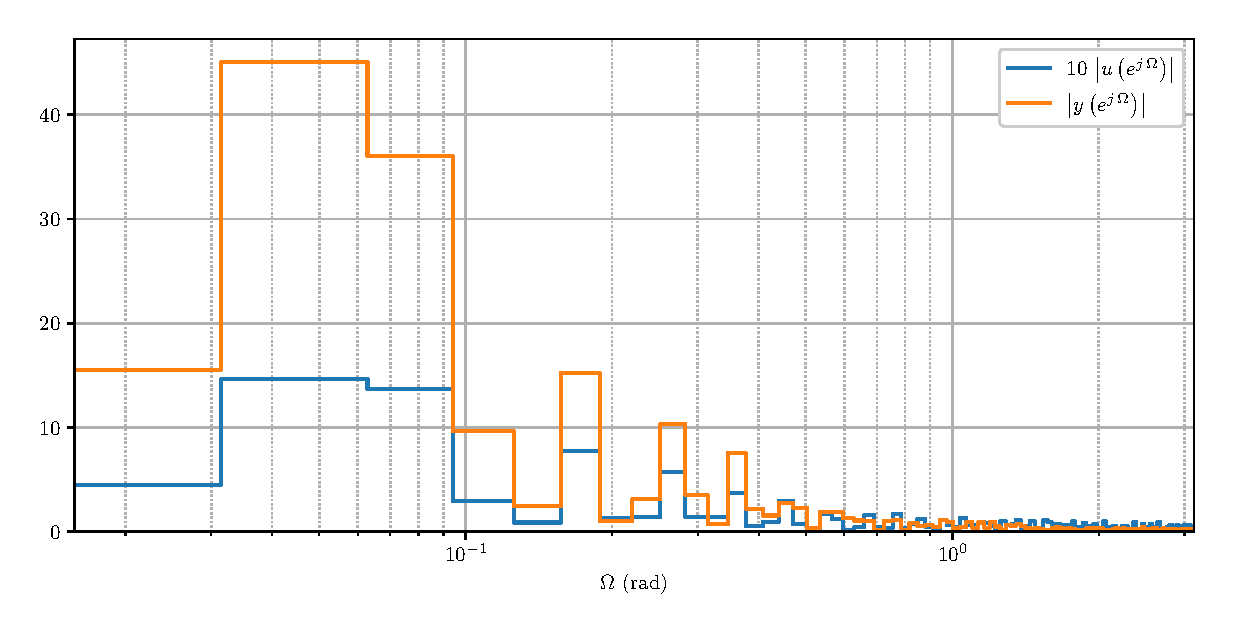
\includegraphics[width=\linewidth]{data_fourier_log}
\end{frame}

\begin{frame}{Identificação - Ordens}
  \newcolumntype{C}{>{\centering\arraybackslash}X}
\setlength{\extrarowheight}{1pt}
\begin{tabularx}{\linewidth}{@{} c *{6}{C} c @{}}
  \toprule
  Classe & $n_a$    & $n_b$    & $n_c$    & $n_d$    & $n_f$    & $n_k$    & Total \\
  \midrule
  ARX    & $[1, 4]$ & $[0, 4]$ & --       & --       & --       & $[1, 4]$ & 80    \\
  ARMAX  & $[1, 4]$ & $[0, 4]$ & $[1, 4]$ & --       & --       & $[1, 4]$ & 320   \\
  OE     & --       & $[0, 4]$ & --       & --       & $[1, 4]$ & $[1, 4]$ & 80    \\
  BJ     & --       & $[0, 4]$ & $[0, 4]$ & $[1, 4]$ & $[1, 4]$ & $[1, 4]$ & 1600  \\
  \midrule
  Total  &          &          &          &          &          &          & 2080  \\
  \bottomrule
\end{tabularx}
\end{frame}

\begin{frame}{Identificação - Resultados por Classe}
  \sisetup{round-precision = 3}
  \newcolumntype{C}{>{\centering\arraybackslash}X}
\setlength{\extrarowheight}{1pt}
\begin{tabularx}{\textwidth}{@{} c c *{4}{C} c c c c @{}}
  \toprule
  \#   & Classe & $n_a$   & $n_b$   & $n_c$   & $n_k$   & $\text{AICc}_v$ & $\text{AICc}_i$ & $J_v$         & $J_i$        \\
  \midrule
  24   & ARX    & \num{2} & \num{1} & --      & \num{1} & \num{79.463 }   & \num{288.142}   & \num{5.801  } & \num{5.750 } \\
  44   & ARX    & \num{3} & \num{1} & --      & \num{1} & \num{80.358 }   & \num{289.971}   & \num{5.556  } & \num{5.740 } \\
  28   & ARX    & \num{2} & \num{2} & --      & \num{1} & \num{80.596 }   & \num{276.503}   & \num{5.589  } & \num{5.276 } \\
  20   & ARX    & \num{2} & \num{0} & --      & \num{1} & \num{80.820 }   & \num{290.423}   & \num{6.384  } & \num{5.910 } \\
  40   & ARX    & \num{3} & \num{0} & --      & \num{1} & \num{81.303 }   & \num{291.572}   & \num{6.074  } & \num{5.875 } \\
  32   & ARX    & \num{2} & \num{3} & --      & \num{1} & \num{82.077 }   & \num{278.289}   & \num{5.410  } & \num{5.264 } \\
  \midrule
  160  & ARMAX  & \num{2} & \num{0} & \num{1} & \num{1} & \num{82.406 }   & \num{292.387}   & \num{6.244  } & \num{5.905 } \\
  240  & ARMAX  & \num{3} & \num{0} & \num{1} & \num{1} & \num{82.440 }   & \num{291.698}   & \num{5.853  } & \num{5.802 } \\
  192  & ARMAX  & \num{2} & \num{2} & \num{1} & \num{1} & \num{83.302 }   & \num{278.685}   & \num{5.579  } & \num{5.277 } \\
  144  & ARMAX  & \num{1} & \num{4} & \num{1} & \num{1} & \num{83.435 }   & \num{299.330}   & \num{5.199  } & \num{5.922 } \\
  112  & ARMAX  & \num{1} & \num{2} & \num{1} & \num{1} & \num{83.574 }   & \num{294.450}   & \num{6.021  } & \num{5.902 } \\
  336  & ARMAX  & \num{4} & \num{1} & \num{1} & \num{1} & \num{84.031 }   & \num{282.669}   & \num{5.277  } & \num{5.337 } \\
  \bottomrule
\end{tabularx}
\end{frame}

\begin{frame}{Identificação - Resultados por Classe}
  \sisetup{round-precision = 3}
  \newcolumntype{C}{>{\centering\arraybackslash}X}
\setlength{\extrarowheight}{1pt}
\begin{tabularx}{\textwidth}{@{} c c *{5}{C} c c c c @{}}
  \toprule
  \#   & Classe & $n_b$   & $n_c$   & $n_d$   & $n_f$   & $n_k$   & $\text{AICc}_v$ & $\text{AICc}_i$ & $J_v$         & $J_i$        \\
  \midrule
  465  & OE     & \num{4} & --      & --      & \num{1} & \num{2} & \num{203.538}   & \num{635.576}   & \num{112.710} & \num{49.103} \\
  469  & OE     & \num{4} & --      & --      & \num{2} & \num{2} & \num{205.126}   & \num{637.238}   & \num{108.924} & \num{48.942} \\
  466  & OE     & \num{4} & --      & --      & \num{1} & \num{3} & \num{208.209}   & \num{688.227}   & \num{126.671} & \num{68.237} \\
  468  & OE     & \num{4} & --      & --      & \num{2} & \num{1} & \num{210.717}   & \num{620.915}   & \num{125.264} & \num{44.195} \\
  470  & OE     & \num{4} & --      & --      & \num{2} & \num{3} & \num{211.195}   & \num{690.408}   & \num{126.771} & \num{68.234} \\
  464  & OE     & \num{4} & --      & --      & \num{1} & \num{1} & \num{211.208}   & \num{622.115}   & \num{136.532} & \num{45.141} \\
  \midrule
  1136 & BJ     & \num{2} & \num{0} & \num{2} & \num{1} & \num{1} & \num{82.909 }   & \num{276.778}   & \num{5.524  } & \num{5.214 } \\
  816  & BJ     & \num{1} & \num{0} & \num{2} & \num{1} & \num{1} & \num{83.040 }   & \num{273.646}   & \num{5.941  } & \num{5.183 } \\
  832  & BJ     & \num{1} & \num{0} & \num{3} & \num{1} & \num{1} & \num{84.041 }   & \num{276.120}   & \num{5.683  } & \num{5.193 } \\
  1456 & BJ     & \num{3} & \num{0} & \num{2} & \num{1} & \num{1} & \num{84.939 }   & \num{277.505}   & \num{5.398  } & \num{5.167 } \\
  1140 & BJ     & \num{2} & \num{0} & \num{2} & \num{2} & \num{1} & \num{85.844 }   & \num{278.965}   & \num{5.521  } & \num{5.214 } \\
  848  & BJ     & \num{1} & \num{0} & \num{4} & \num{1} & \num{1} & \num{86.957 }   & \num{274.874}   & \num{5.677  } & \num{5.083 } \\
  \bottomrule
\end{tabularx}
\end{frame}

\begin{frame}{Identificação - Resultados Gerais}
  \sisetup{round-precision = 3}
  \newcolumntype{C}{>{\centering\arraybackslash}X}
\setlength{\extrarowheight}{1pt}
\begin{tabularx}{\textwidth}{@{} c c *{5}{C} c c c c @{}}
  \toprule
  \#   & Classe & $n_a$   & $n_b$   & $n_c$   & $n_d$   & $n_f$   & $\text{AICc}_v$ & $\text{AICc}_i$ & $J_v$  & $J_i$       \\
  \midrule
  24   & ARX    & \num{2} & \num{1} &  --     &  --       &  --   & \num{79.463} & \num{288.142} & \num{5.801} & \num{5.750} \\
  44   & ARX    & \num{3} & \num{1} &  --     &  --       &  --   & \num{80.358} & \num{289.971} & \num{5.556} & \num{5.740} \\
  28   & ARX    & \num{2} & \num{2} &  --     &  --       &  --   & \num{80.596} & \num{276.503} & \num{5.589} & \num{5.276} \\
  20   & ARX    & \num{2} & \num{0} &  --     &  --       &  --   & \num{80.820} & \num{290.423} & \num{6.384} & \num{5.910} \\
  40   & ARX    & \num{3} & \num{0} &  --     &  --       &  --   & \num{81.303} & \num{291.572} & \num{6.074} & \num{5.875} \\
  32   & ARX    & \num{2} & \num{3} &  --     &  --       &  --   & \num{82.077} & \num{278.289} & \num{5.410} & \num{5.264} \\
  64   & ARX    & \num{4} & \num{1} &  --     &  --       &  --   & \num{82.145} & \num{288.495} & \num{5.419} & \num{5.611} \\
  160  & ARMAX  & \num{2} & \num{0} & \num{1} &  --       &  --   & \num{82.406} & \num{292.387} & \num{6.244} & \num{5.905} \\
  240  & ARMAX  & \num{3} & \num{0} & \num{1} &  --       &  --   & \num{82.440} & \num{291.698} & \num{5.853} & \num{5.802} \\
  1136 & BJ     &  --     & \num{2} & \num{0} & \num{2} & \num{1} & \num{82.909} & \num{276.778} & \num{5.524} & \num{5.214} \\
  816  & BJ     &  --     & \num{1} & \num{0} & \num{2} & \num{1} & \num{83.040} & \num{273.646} & \num{5.941} & \num{5.183} \\
  36   & ARX    & \num{2} & \num{4} &  --     &  --       &  --   & \num{83.283} & \num{281.484} & \num{5.179} & \num{5.297} \\
  192  & ARMAX  & \num{2} & \num{2} & \num{1} &  --       &  --   & \num{83.302} & \num{278.685} & \num{5.579} & \num{5.277} \\
  % 60   & ARX    & \num{4} & \num{0} &  --     &  --       &  --   & \num{83.403} & \num{291.217} & \num{5.995} & \num{5.784} \\
  % 144  & ARMAX  & \num{1} & \num{4} & \num{1} &  --       &  --   & \num{83.435} & \num{299.330} & \num{5.199} & \num{5.922} \\
  % 112  & ARMAX  & \num{1} & \num{2} & \num{1} &  --       &  --   & \num{83.574} & \num{294.450} & \num{6.021} & \num{5.902} \\
  % 48   & ARX    & \num{3} & \num{2} &  --     &  --       &  --   & \num{83.698} & \num{278.625} & \num{5.634} & \num{5.275} \\
  % 336  & ARMAX  & \num{4} & \num{1} & \num{1} &  --       &  --   & \num{84.031} & \num{282.669} & \num{5.277} & \num{5.337} \\
  % 832  & BJ     &  --     & \num{1} & \num{0} & \num{3} & \num{1} & \num{84.041} & \num{276.120} & \num{5.683} & \num{5.193} \\
  % 52   & ARX    & \num{3} & \num{3} &  --     &  --       &  --   & \num{84.774} & \num{280.442} & \num{5.376} & \num{5.263} \\
  \bottomrule
\end{tabularx}
  $n_k = 1$ em todos os modelos
\end{frame}

\begin{frame}{Comparação - Resposta em Frequência - $G(q)$}
  \centering
  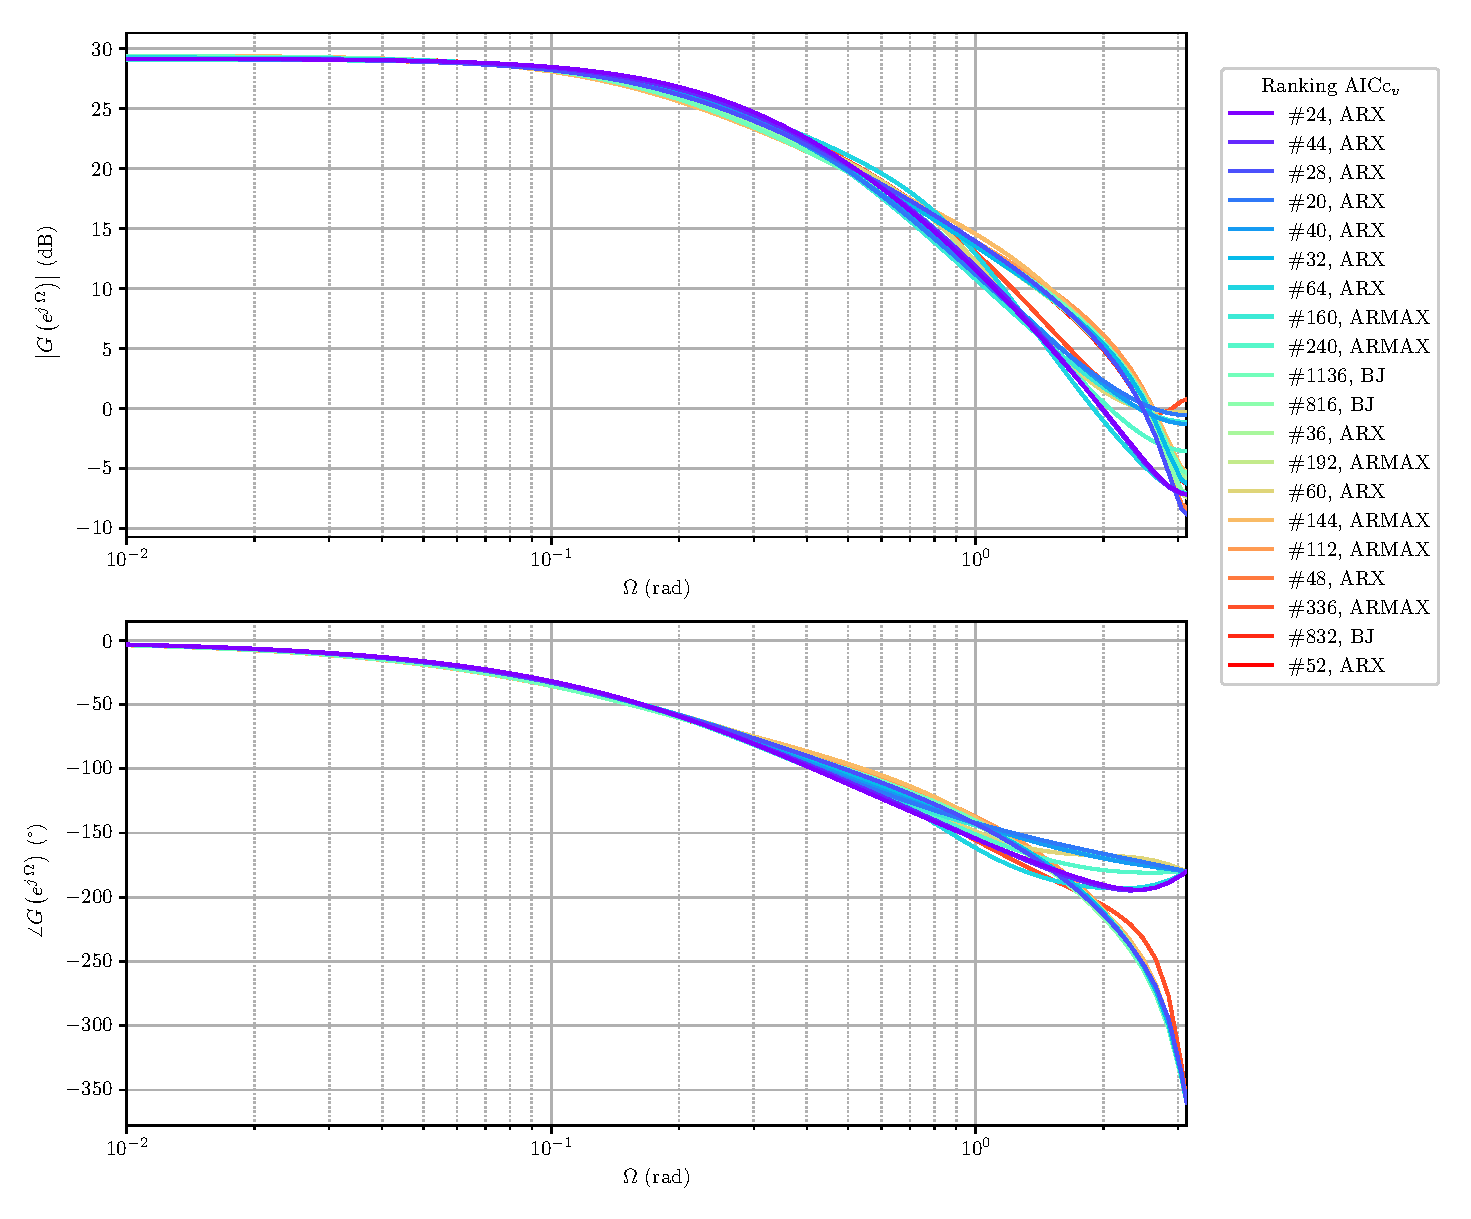
\includegraphics[width=.9\linewidth]{bode_G_AICCv}
\end{frame}

\begin{frame}{Comparação - Resposta em Frequência - $H(q)$}
  \centering
  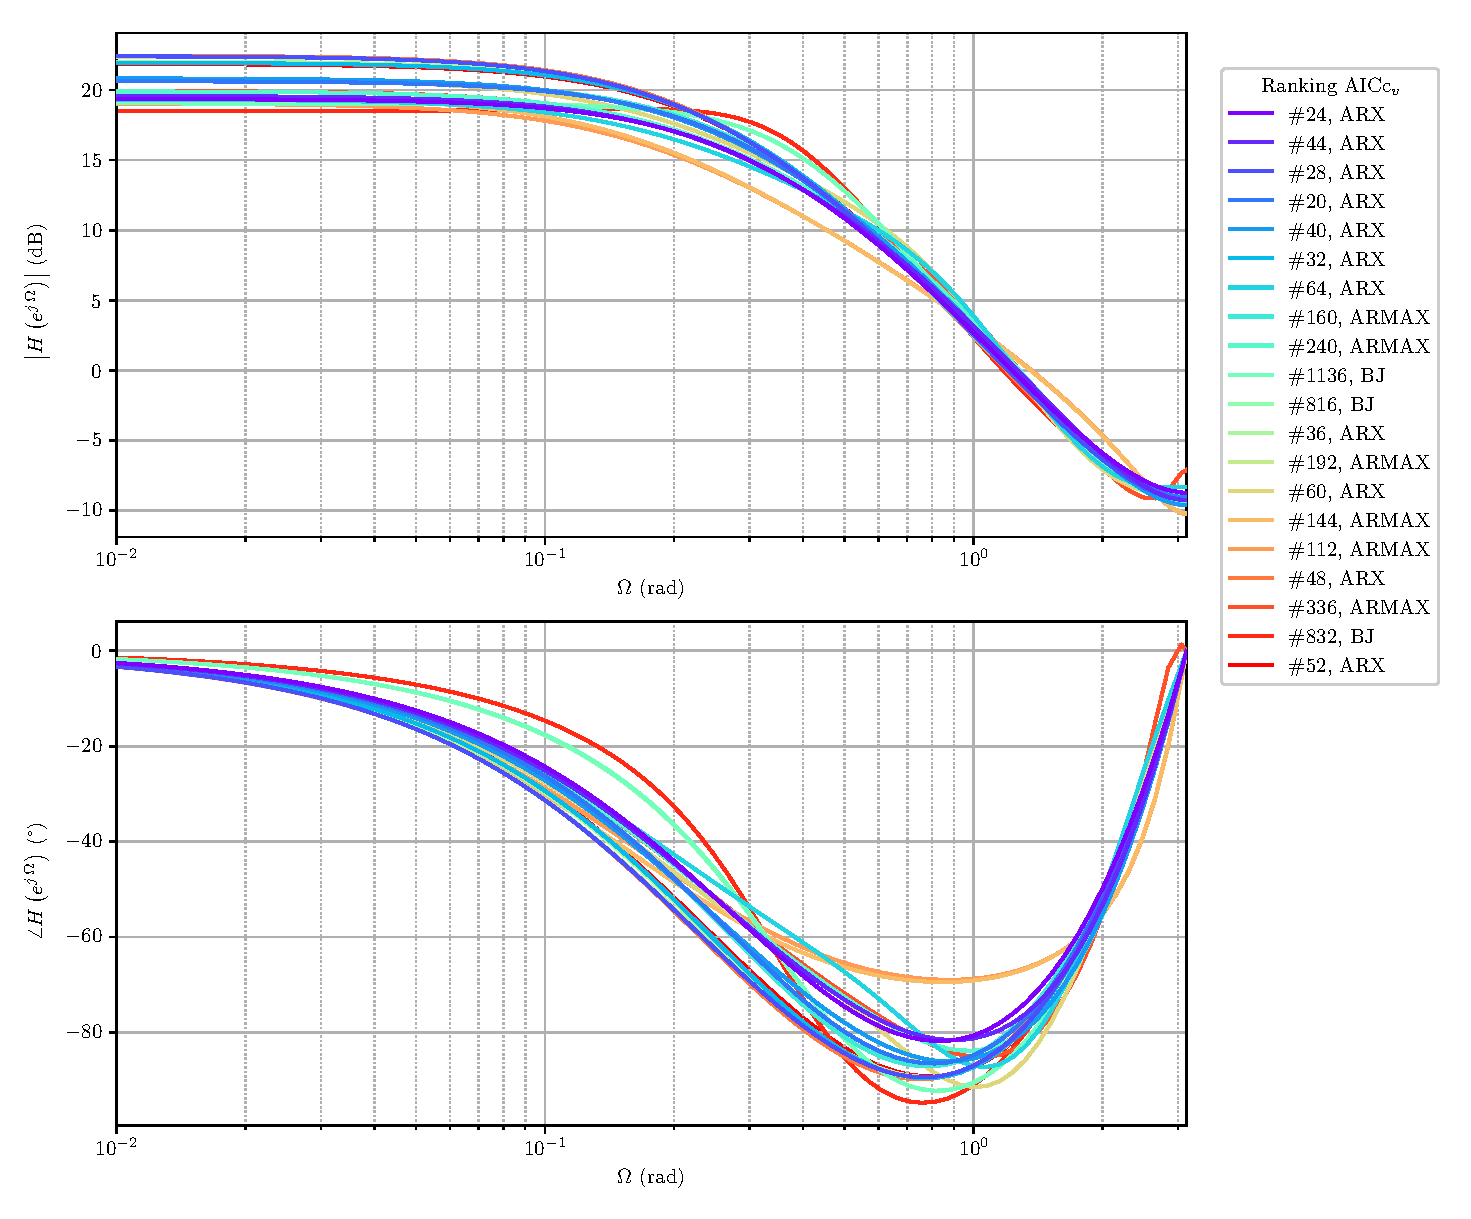
\includegraphics[width=.9\linewidth]{bode_H_AICCv}
\end{frame}

\begin{frame}{Comparação - Predições}
  \begin{gather}
    \hat{y}(t) = L_u(q) \, u(t) + L_y(q) \, y(t)
    \\
    L_u(q) = \dfrac{G(q)}{H(q)}
    \qquad
    L_y(q) = 1 - \dfrac{1}{H(q)}
    \end{gather}
  \centering
  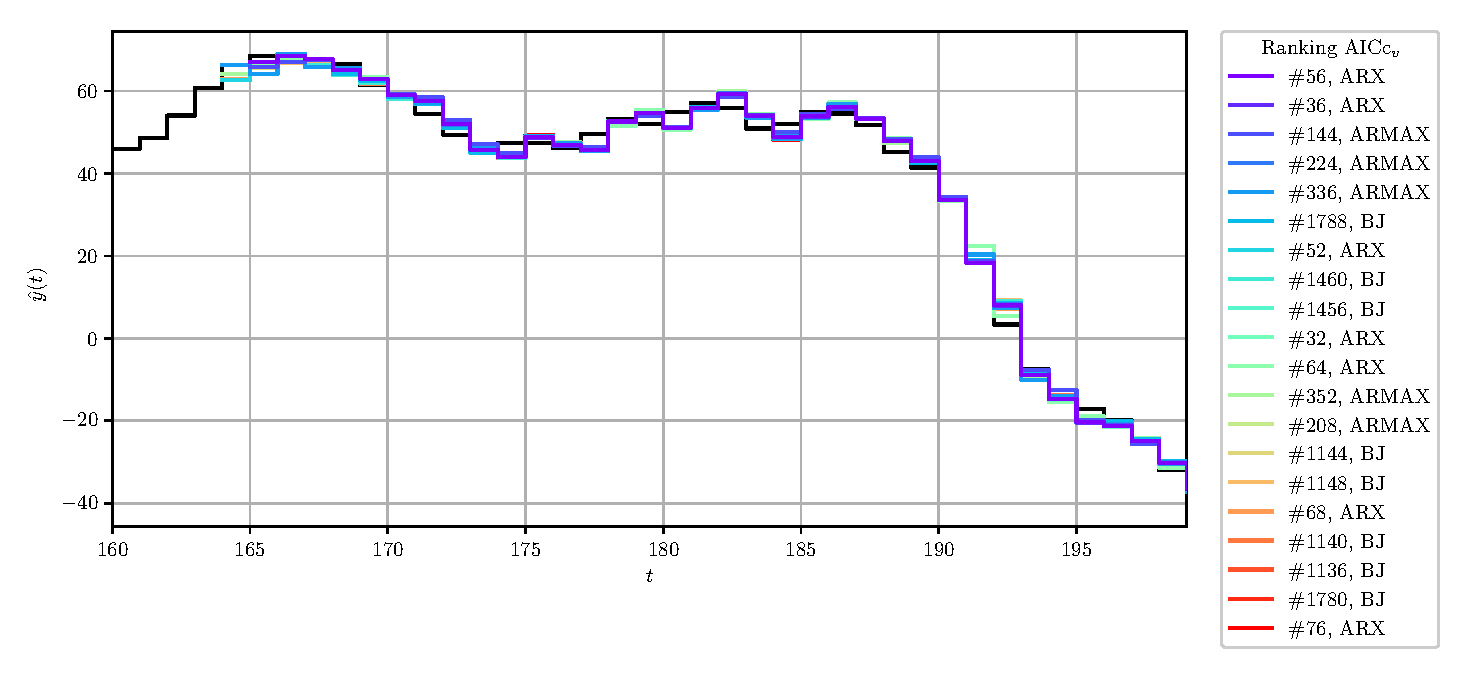
\includegraphics[width=.9\linewidth]{prediction_AICCv}
\end{frame}

\begin{frame}{Comparação - Resíduos}
  \begin{align}
    \varepsilon(t)
    &= y(t) - \hat{y}(t)
    \\
    &= \dfrac{y(t) - G(q) \Prod u(t)}{H(q)}
  \end{align}
  \centering
  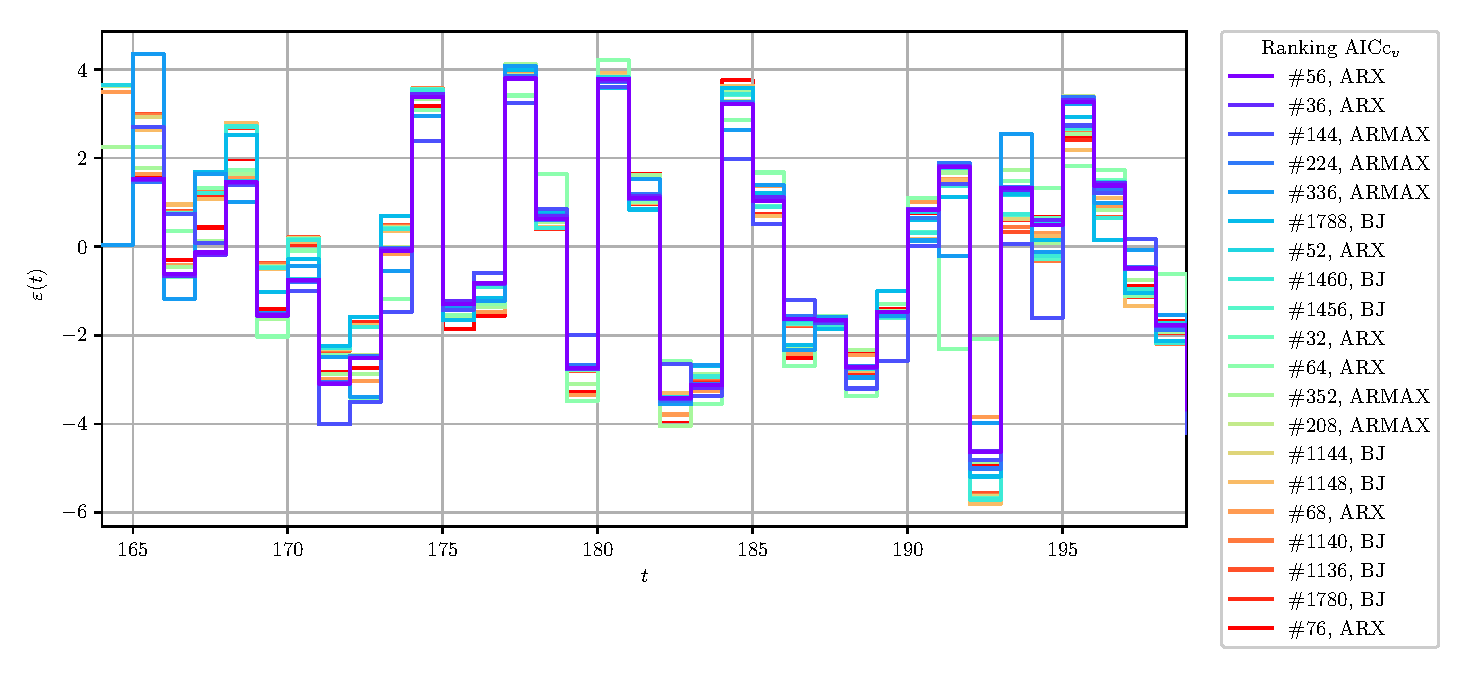
\includegraphics[width=.9\linewidth]{residue_AICCv}
\end{frame}

\begin{frame}{Comparação - Resíduos - Autocorrelação}
  \begin{gather}
    R_{\varepsilon}(\Delta t) = \sum_{t=-N}^{N} \varepsilon(t) \Prod \varepsilon(t + \Delta t)
  \end{gather}
  \centering
  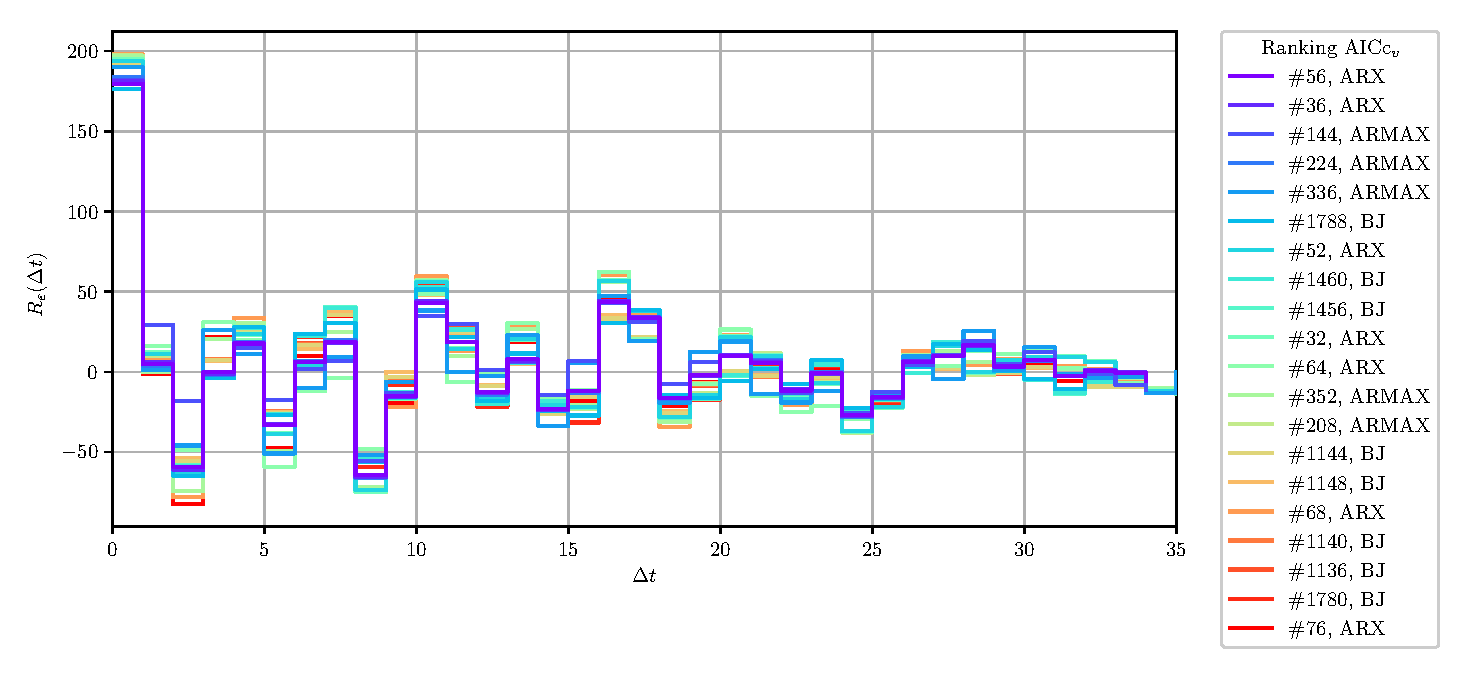
\includegraphics[width=.9\linewidth]{residue_autocorrelation_AICCv}
\end{frame}

\begin{frame}{Sistema Verdadeiro}
  \begin{align}
    G_0(q) &= \dfrac{                   \num{2} \Prod q^2 + \num{2} \Prod q      - \num{1.5}                    }{q^3 - \num{1.4} \Prod q^2    + \num{0.48} \Prod q     }
    \\
           &= \dfrac{q^{-1} \Prod \left(\num{2}           + \num{2} \Prod q^{-1} - \num{1.5} \Prod q^{-2}\right)}{1   - \num{1.4} \Prod q^{-1} + \num{0.48} \Prod q^{-2}}
    \\
    H_0(q) &= \dfrac{q^3}{q^3 - \num{1.4} \Prod q^2    + \num{0.48} \Prod q     }
    \\
           &= \dfrac{1  }{1   - \num{1.4} \Prod q^{-1} + \num{0.48} \Prod q^{-2}}
  \end{align}
  \pause
  Menor Modelo de Ordem Completa:\\
  ARX com $n_a=2$, $n_b=2$, e $n_k=1$
  \begin{align}
    A(q) &= 1 + a_1 \Prod q^{-1} + a_2 \Prod q^{-2}
    \\
    B(q) &= q^{-1} \Prod \left(b_0 + b_1 \Prod q^{-1} + b_2 \Prod q^{-2}\right)
  \end{align}
\end{frame}

\begin{frame}{Menor Modelo de Ordem Completa}
  ARX com $n_a=2$, $n_b=2$, e $n_k=1$ equivale ao modelo \#28
  \begin{align}
    A_{28}(q) &= 1   - \num{1.40683412} \Prod q^{-1} + \num{0.48261202} \Prod q^{-2}
    \\
    B_{28}(q) &= q^{-1} \Prod \left(\num{2.16246556} + \num{1.61084338} \Prod q^{-1} - \num{1.6016382} \Prod q^{-2}\right)
  \end{align}
  \begin{gather}
    \text{AICc}_v = \num{80.820}
    \qquad
    \text{AICc}_i = \num{290.423}
    \qquad
    J_v = \num{6.384}
    \qquad
    J_i = \num{5.910}
  \end{gather}
  \vspace{-20pt}
  \begin{align}
    G_{28}(q) &= \dfrac{                   \num{2.16246556} \Prod q^2 + \num{1.61084338} \Prod q      - \num{1.6016382}                    }{q^3 - \num{1.40683412} \Prod q^2    + \num{0.48261202} \Prod q     }
    \\
    H_{28}(q) &= \dfrac{q^3}{q^3 - \num{1.40683412} \Prod q^2    + \num{0.48261202} \Prod q     }
  \end{align}
  \pause
  \vspace{-15pt}
  \begin{align}
    G_0(q) &= \dfrac{                   \num{2} \Prod q^2 + \num{2} \Prod q      - \num{1.5}                    }{q^3 - \num{1.4} \Prod q^2    + \num{0.48} \Prod q     }
    \\
    H_0(q) &= \dfrac{q^3}{q^3 - \num{1.4} \Prod q^2    + \num{0.48} \Prod q     }
  \end{align}
\end{frame}

\begin{frame}{Menor Modelo de Ordem Completa - Previsão}
  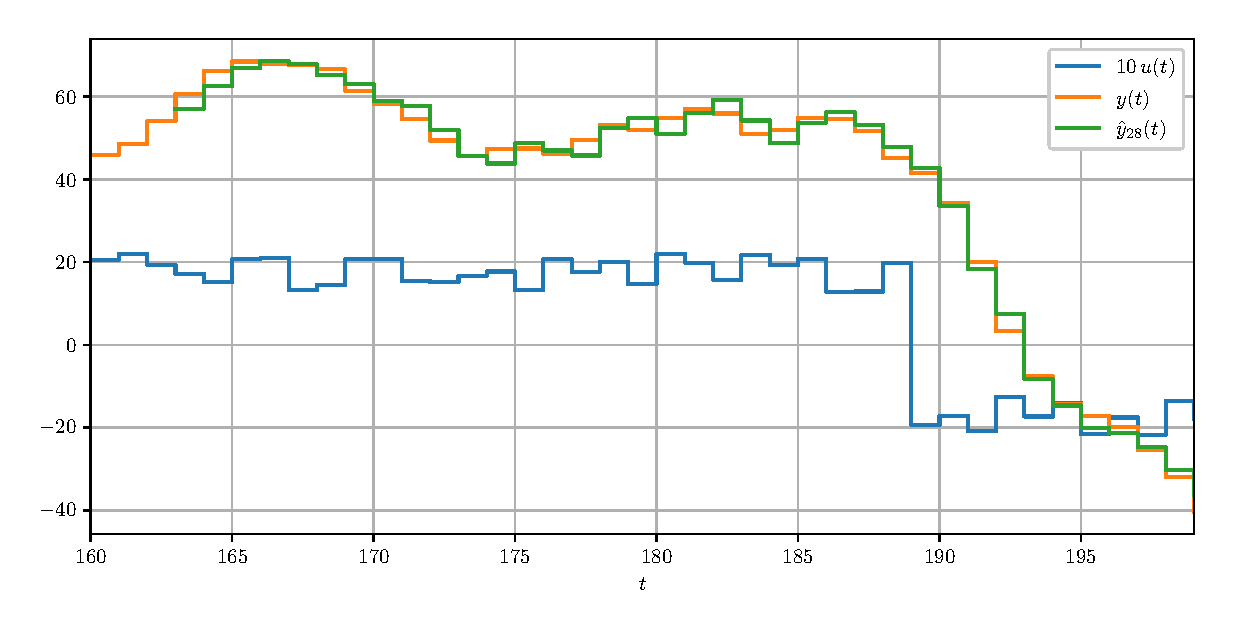
\includegraphics[width=\linewidth]{y_p_28}
  \begin{equation}
    J_v = \num{6.384}
  \end{equation}
\end{frame}

\begin{frame}{Menor Modelo de Ordem Completa - Resposta em Frequência - $G(q)$}
  \centering
  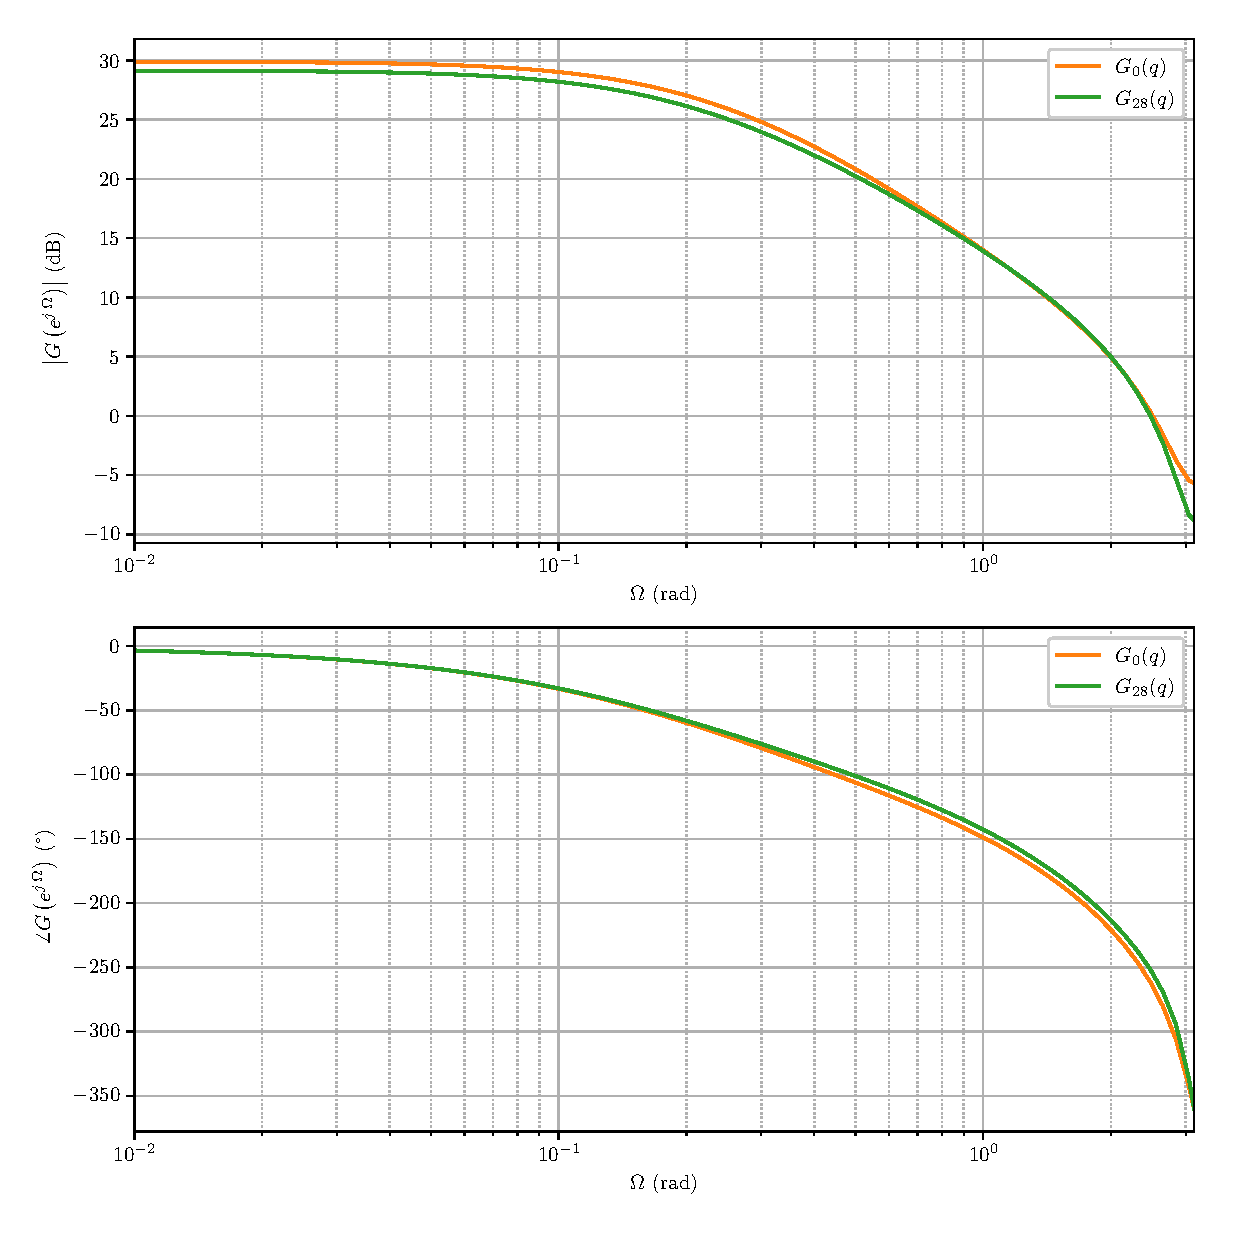
\includegraphics[width=0.7\linewidth]{bode_G_28}
\end{frame}

\begin{frame}{Menor Modelo de Ordem Completa - Resposta em Frequência - $H(q)$}
  \centering
  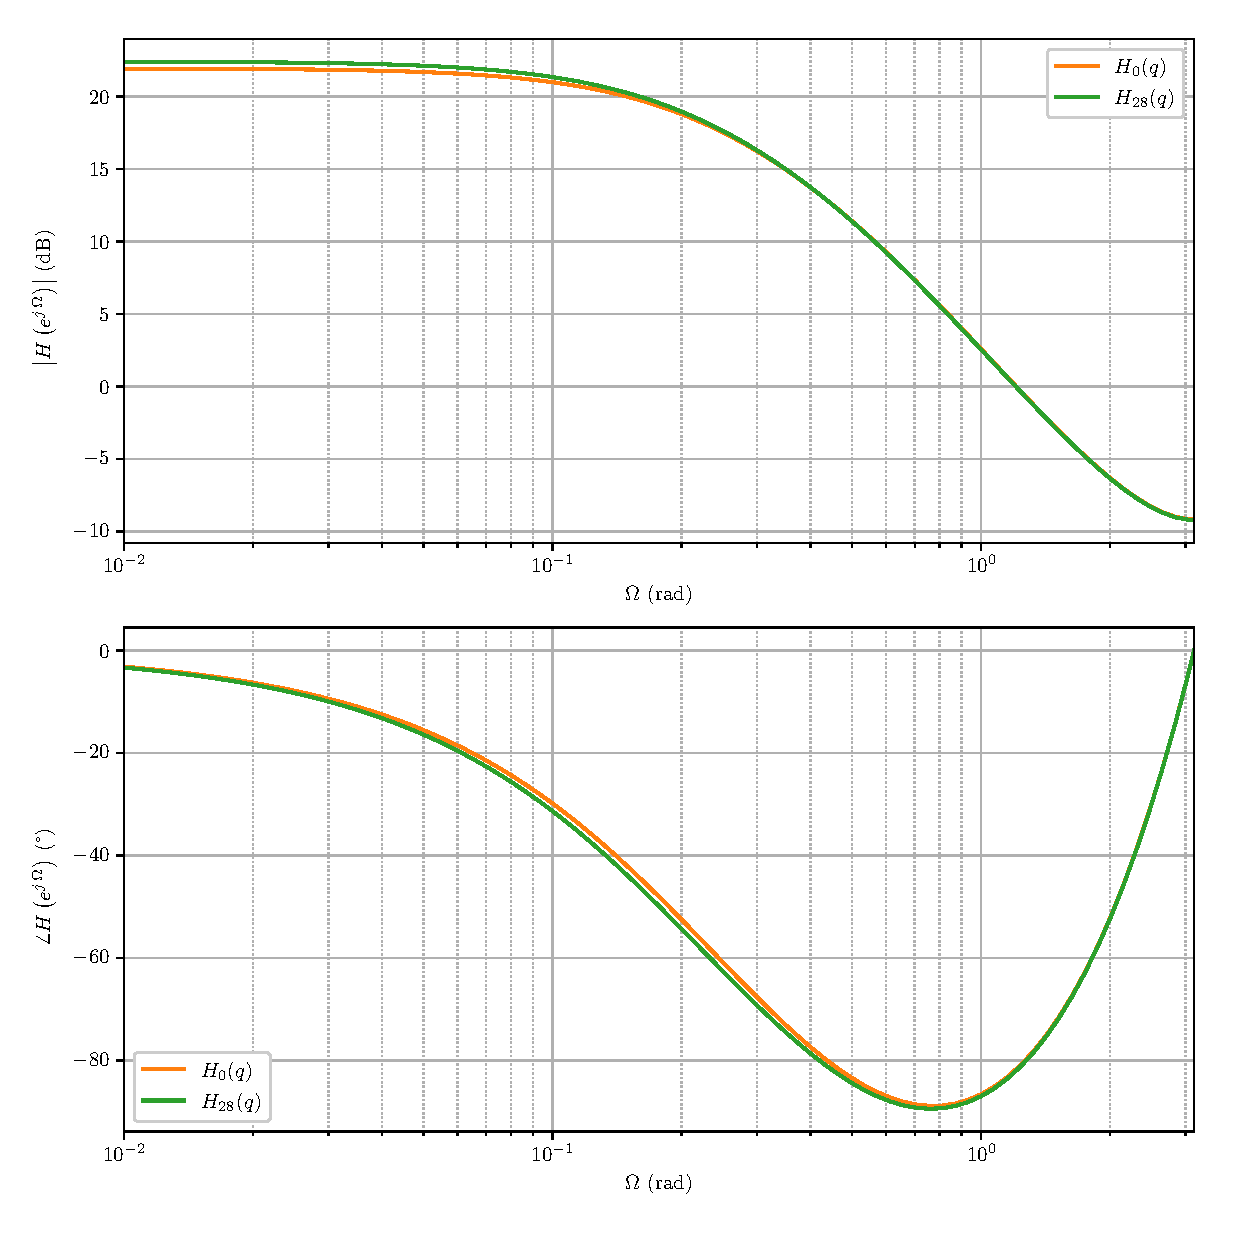
\includegraphics[width=0.7\linewidth]{bode_H_28}
\end{frame}

{
\setbeamertemplate{navigation symbols}{}
\againframe[noframenumbering]{frame:title}
}

\end{document}